\chapter{Systems diagrams and software}
\label{ap:Algorithms}
\graphicspath{{Appendix4/Appendix4figures/}}

\section{Software}
The Git repository for this complete system can be found at\\https://github.com/DriesSmit/AutoTestMarker/tree/master/Software.

\section{Interface}
The software's main interface and clash list are show in Figure \ref{fig:mainInterface} and Figure \ref{fig:clashInterface}, respectively.

\begin{figure}
  \centering
  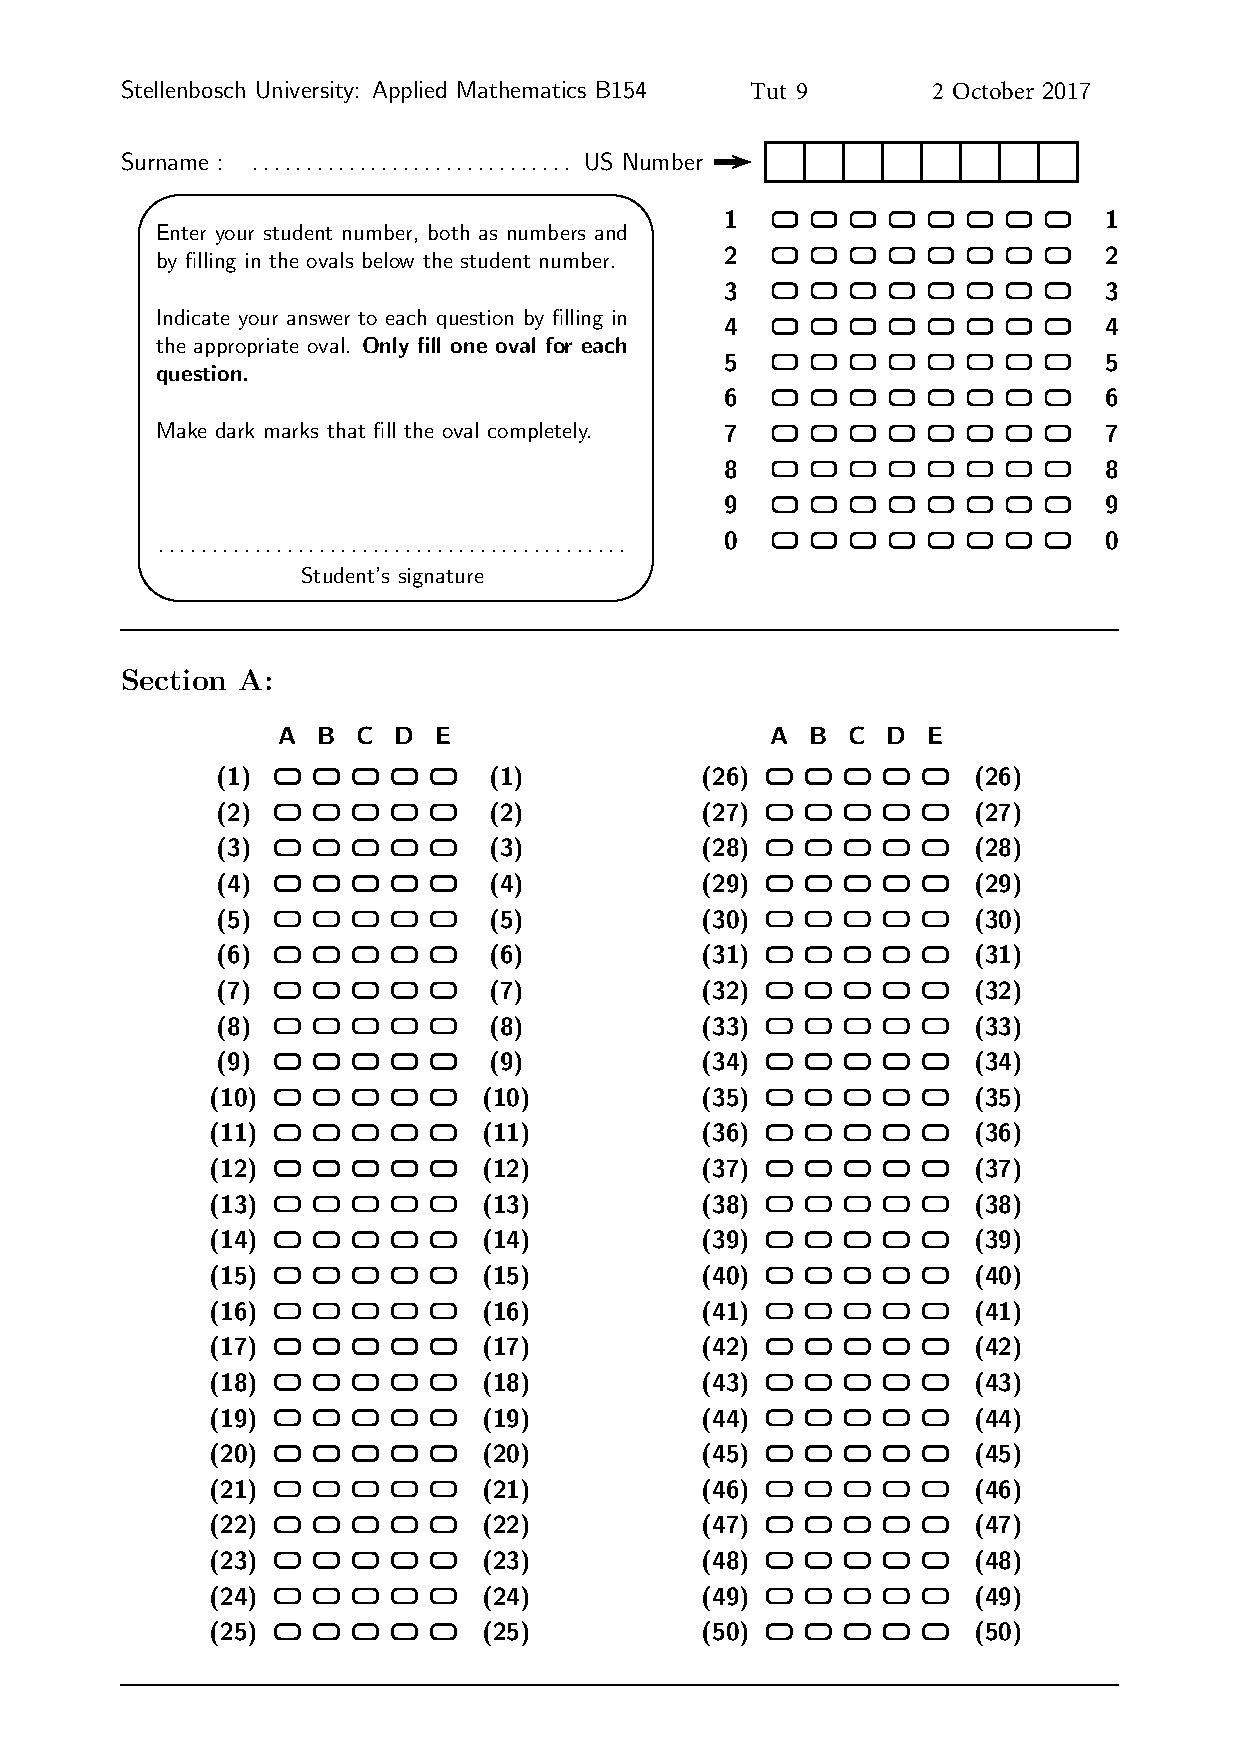
\includegraphics[width=14.2cm]{mainInterface}\\
  \caption{Main interface of the test grader.}
  \label{fig:mainInterface}
\end{figure}

\begin{figure}
  \centering
  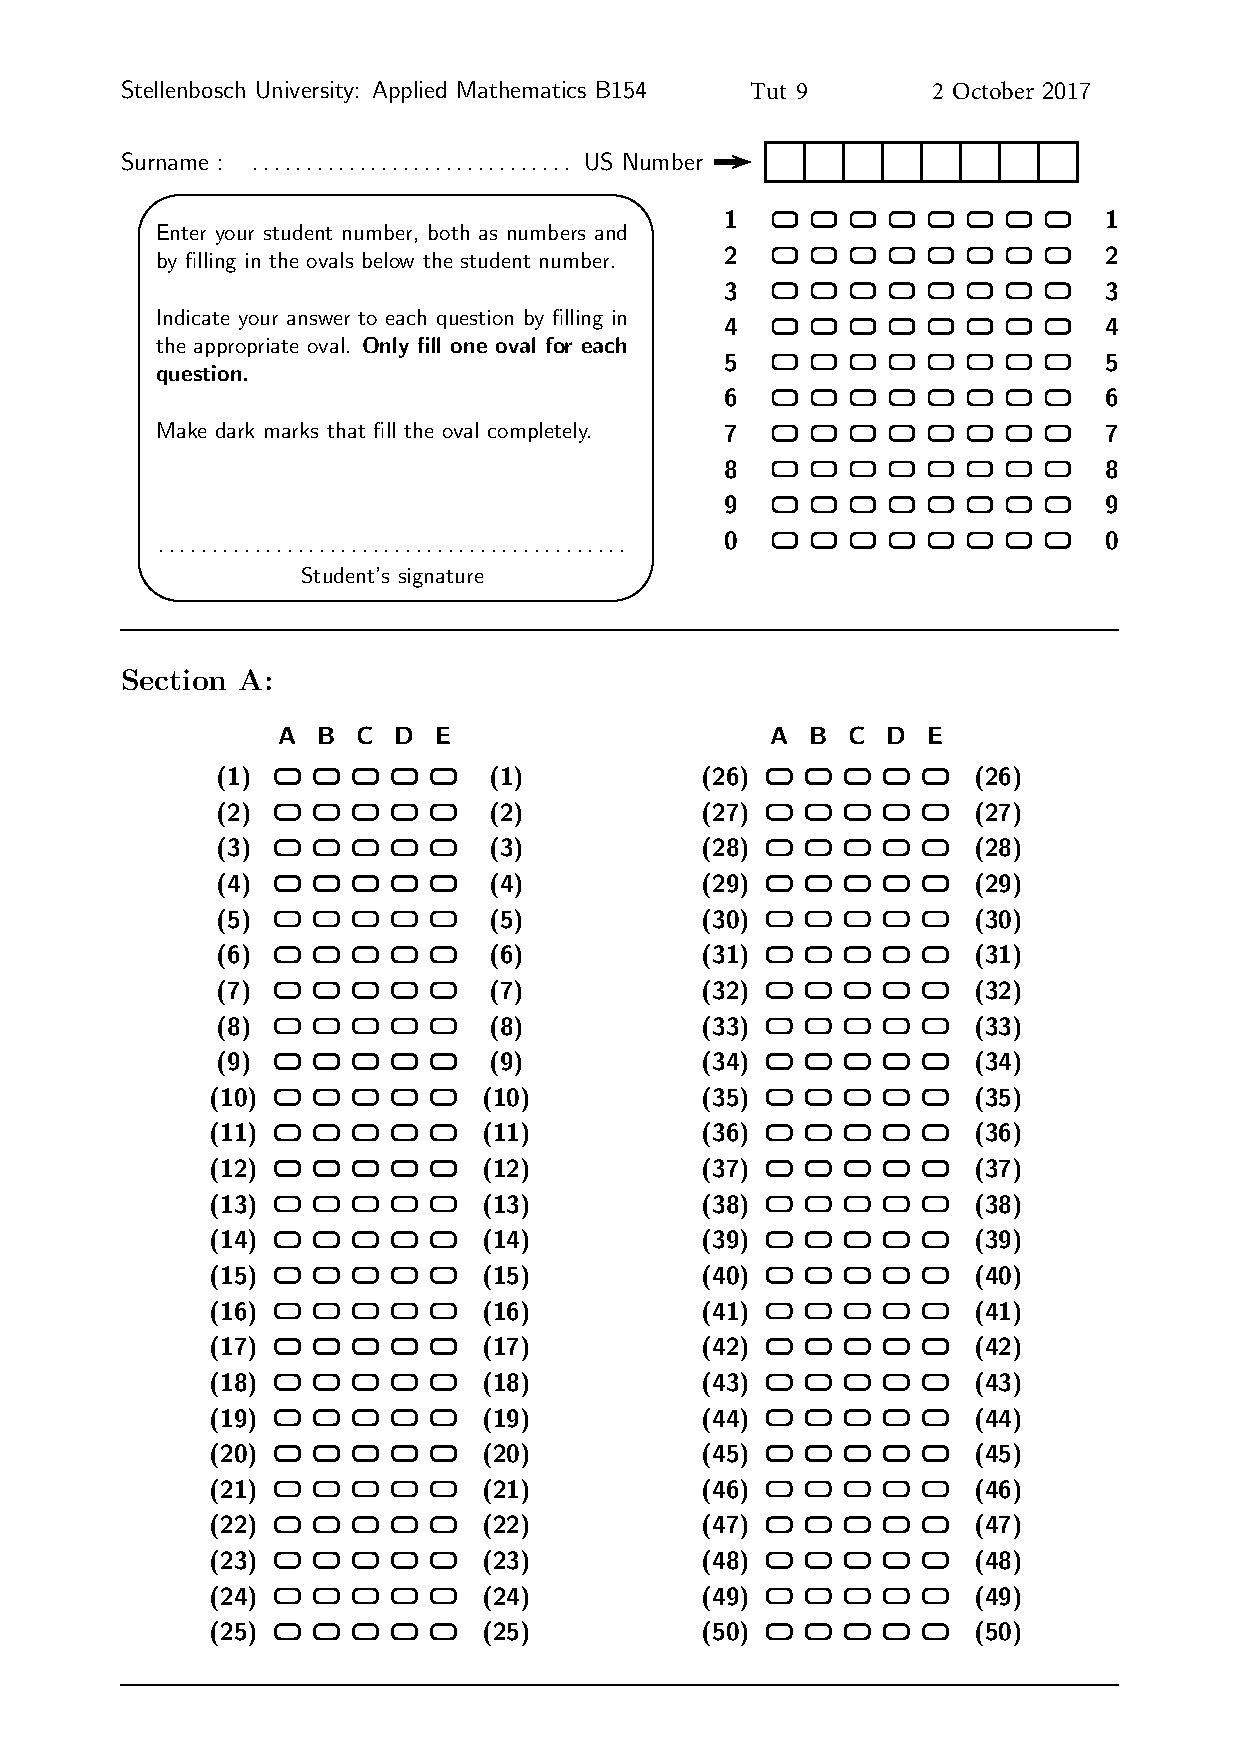
\includegraphics[width=14cm]{clashInterface}\\
  \caption{Clash list interface of the test grader.}
  \label{fig:clashInterface}
\end{figure}

\section{Templates}

The original template is shown in Figure \ref{fig:template1}. 
\begin{figure}
  \centering
  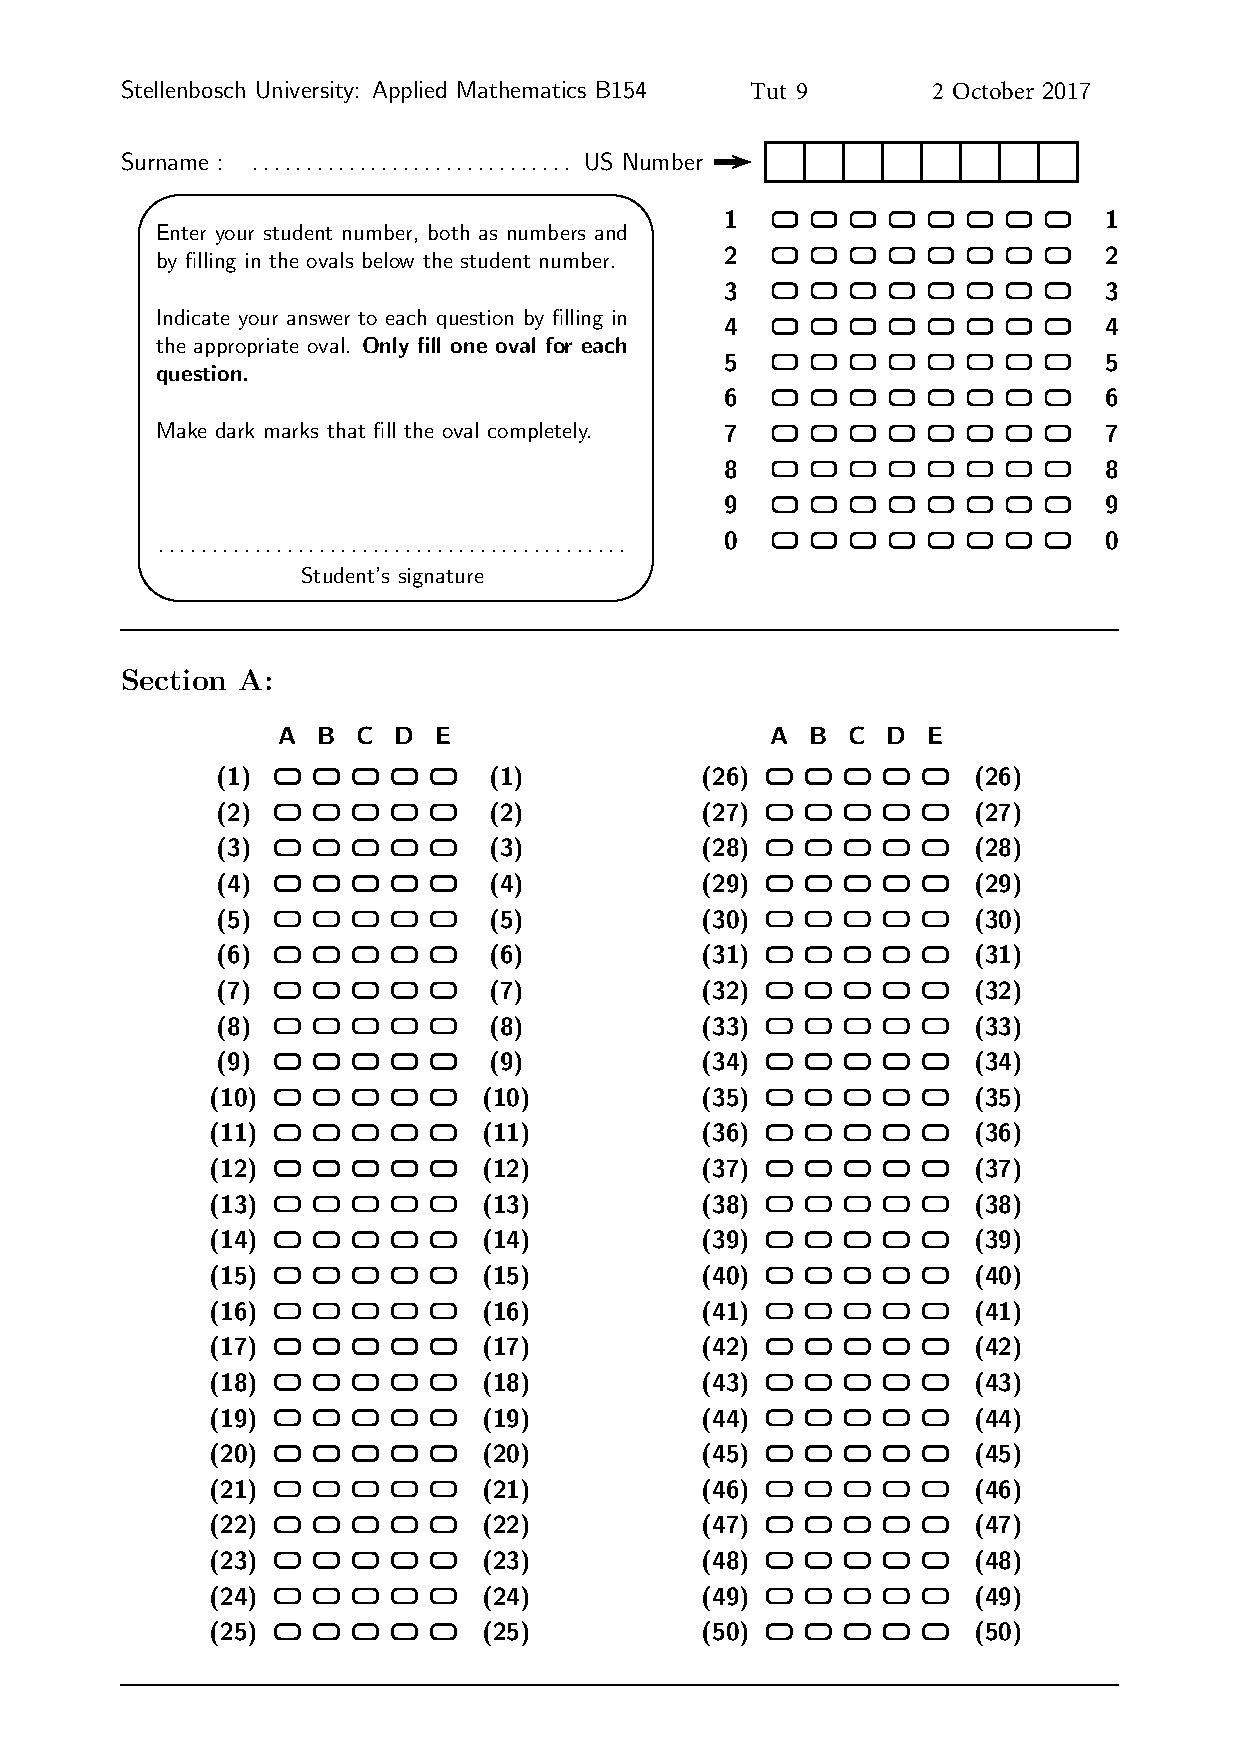
\includegraphics[width=12cm]{template1}\\
  \caption{Original template focussed on numbered answered questions.}
  \label{fig:template1}
\end{figure}
Two additional templates have also been developed and implemented for the department. These templates provides the option of grading numbered answered questions as well as multiple choice questions. These templates are shown in Figure \ref{fig:template2} and Figure \ref{fig:template3}.

\begin{figure}
  \centering
  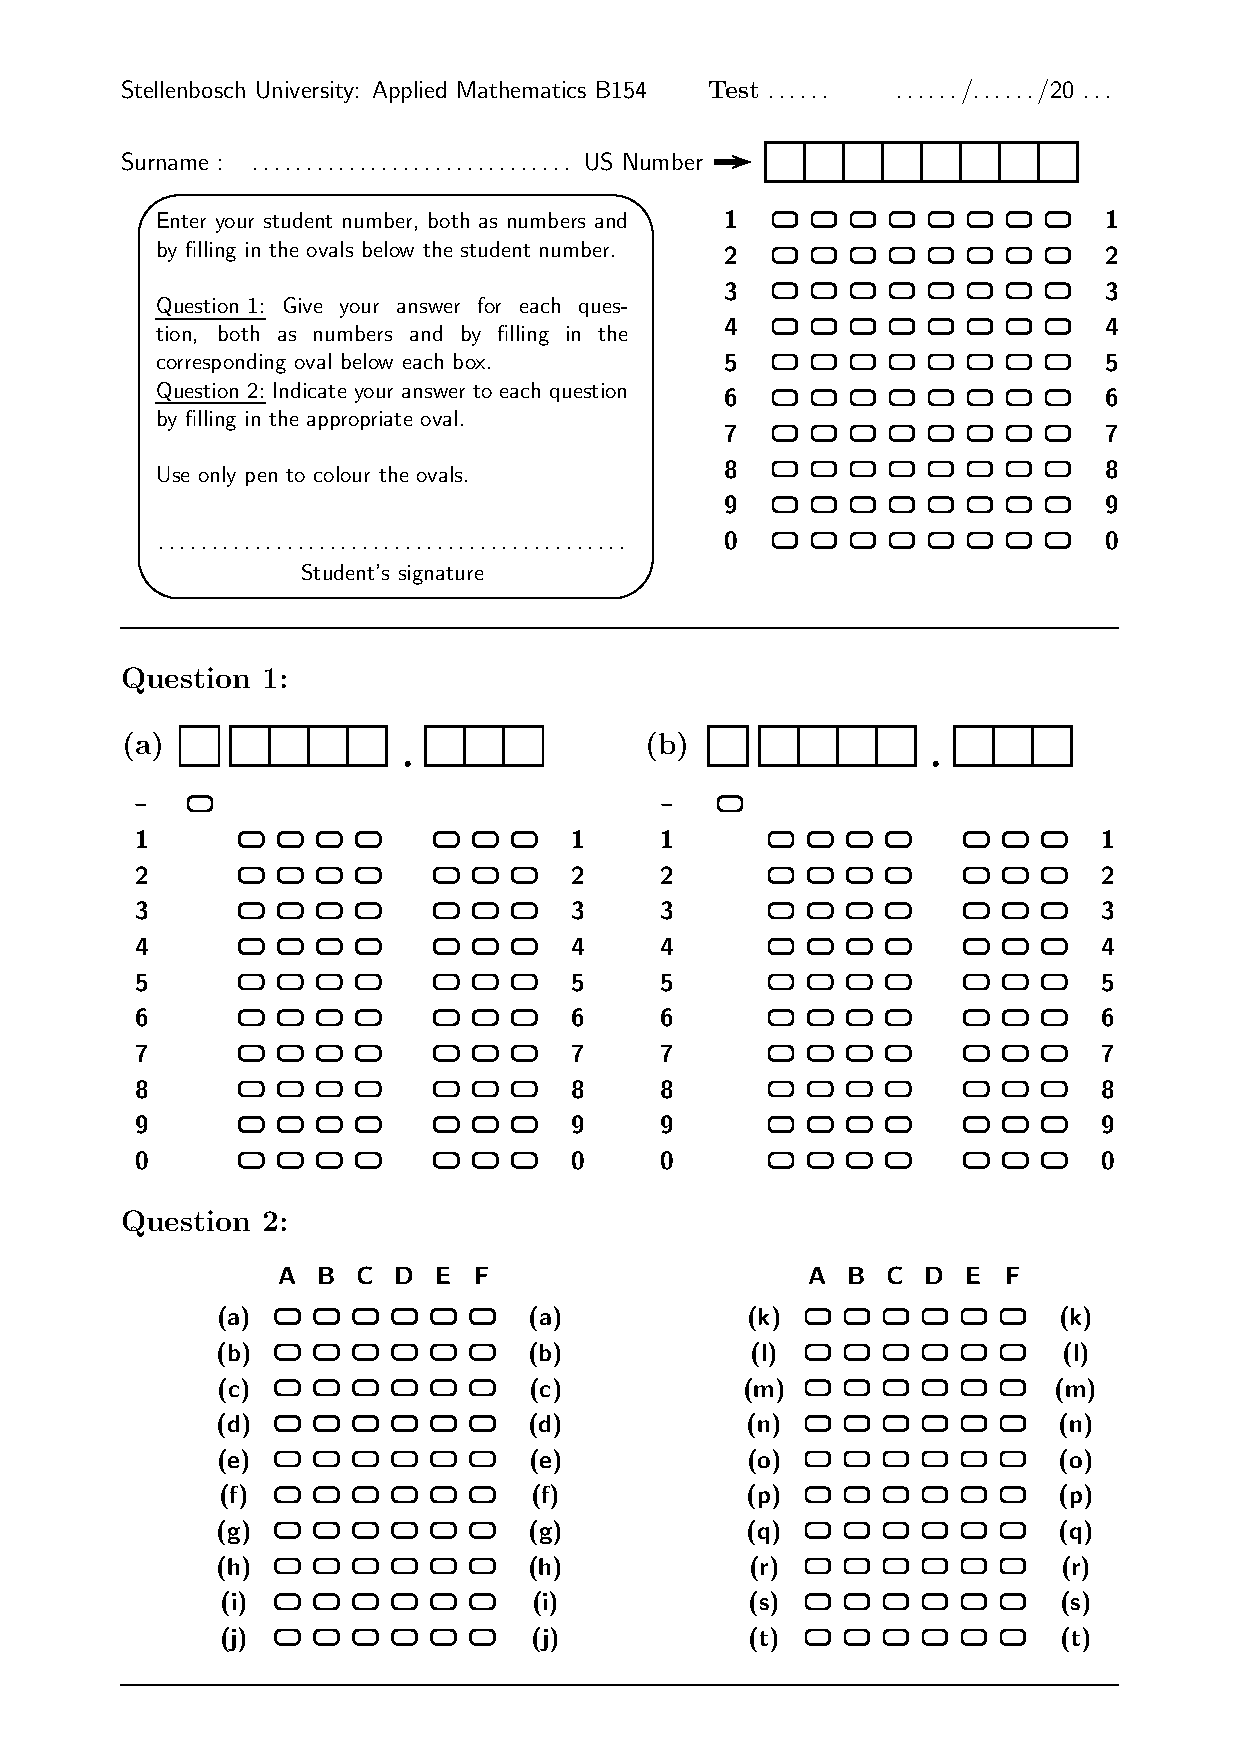
\includegraphics[width=12cm]{template2}\\
  \caption{Template allowing for numbered and multiple choice answers.}
  \label{fig:template2}
\end{figure}

\begin{figure}
  \centering
  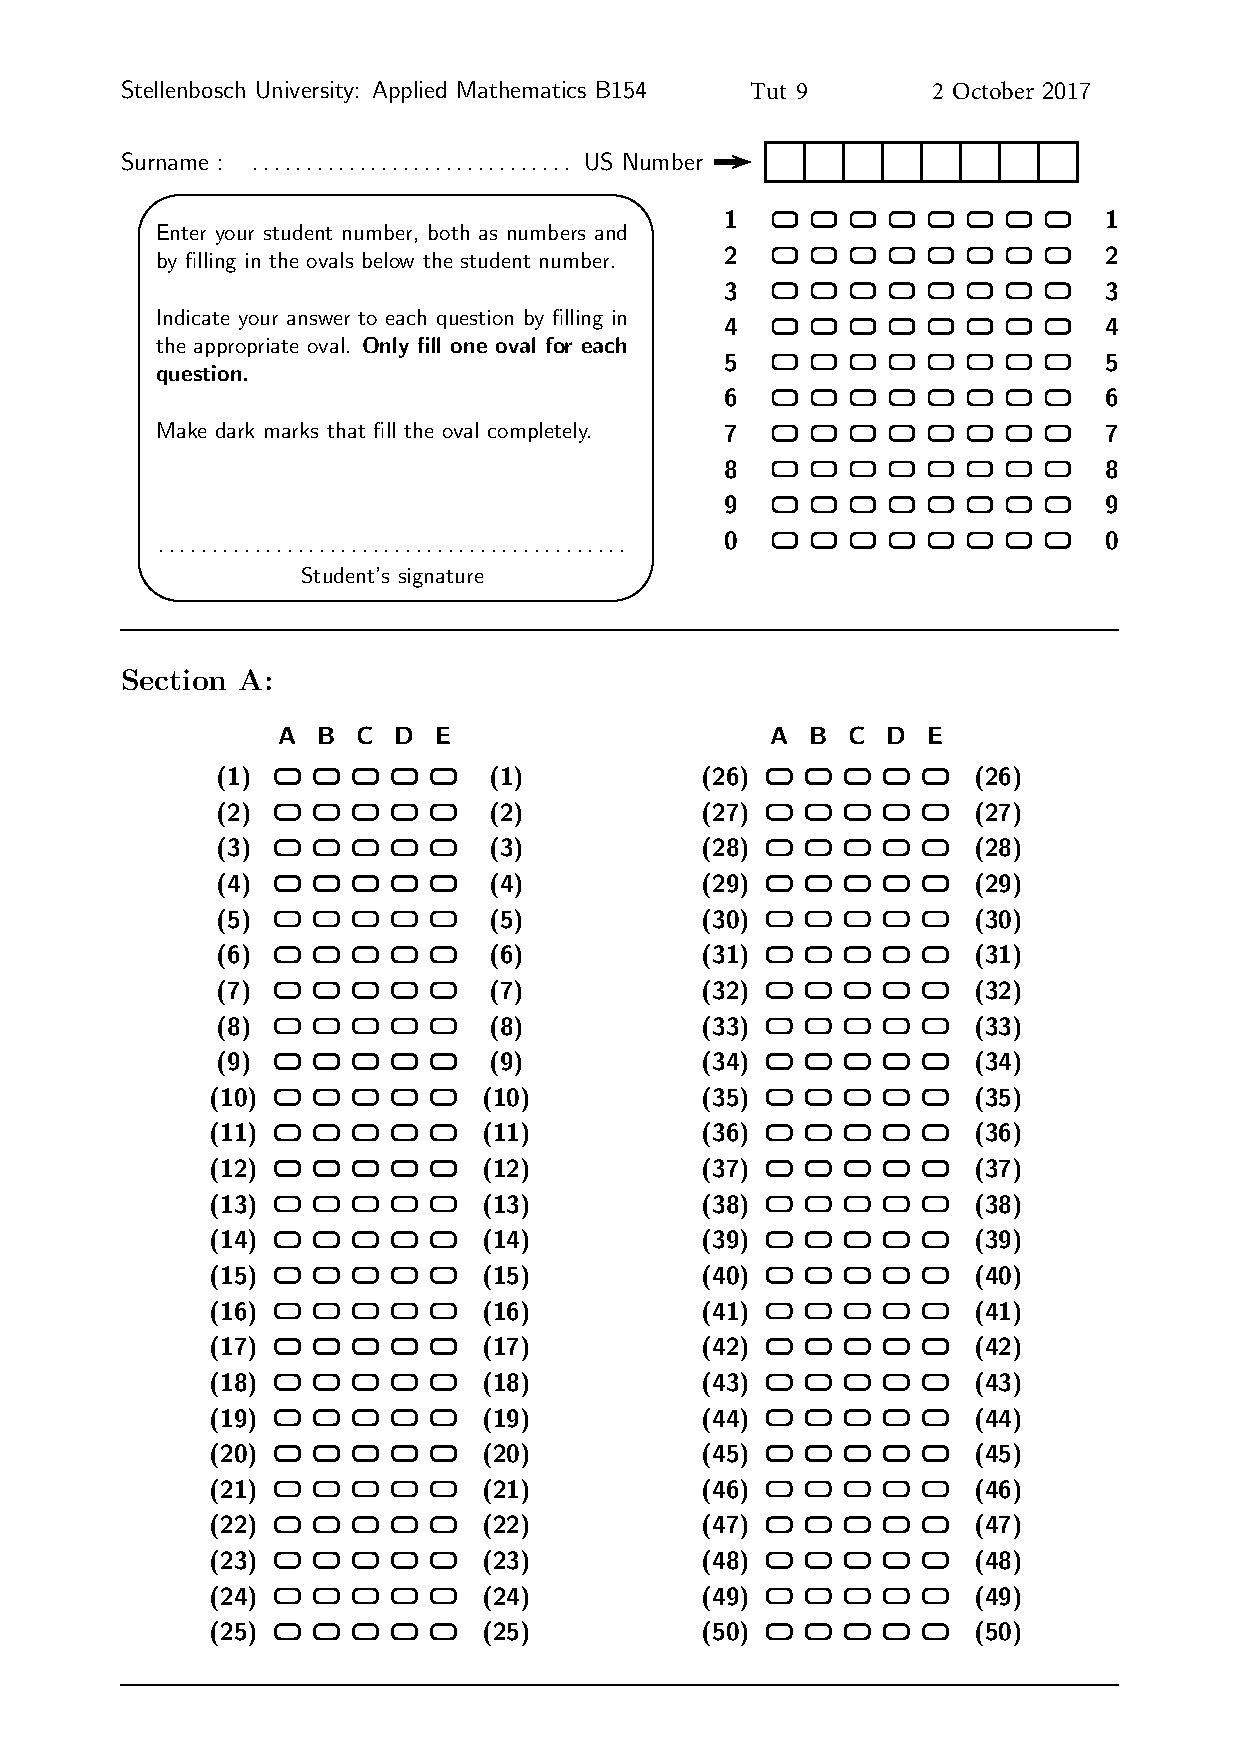
\includegraphics[width=12cm]{template3}\\
  \caption{Template focussed solely on multiple choice type questions.}
  \label{fig:template3}
\end{figure}

%\section{DCNN TensorFlow setup}
%The DCNN structural setup diagram is shown in Figure \ref{fig:DCNN}. This structure was directly used as constructed by the TensorFlow team. Alterations to the input and output methods where made to increase the accuracy of grading characters on a test sheets.

%\begin{figure}
%  \centering
%  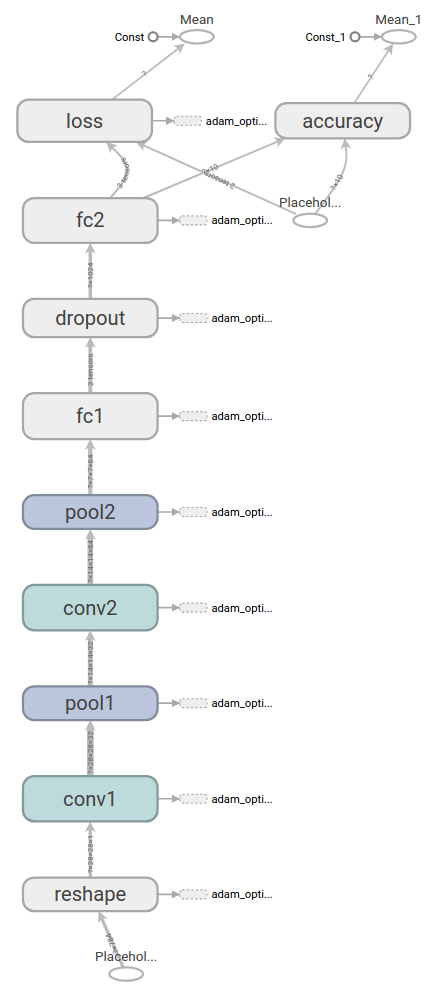
\includegraphics[width=7cm]{DCNN}\\
%  \caption{DCNN structural set up diagram, from \citet{Tensor}}
%  \label{fig:DCNN}
%\end{figure}